% ELT-1031 Lab 06 -- RC Transient Response
% Showcase for phelanlab.cls.
% Build: latexmk phelan-lab06.tex   (the .latexmkrc selects LuaLaTeX)
% Plot data: python3 -I make-plot-data.py  (data/*.xlsx -> data/*.dat)
\documentclass{phelanlab}

\graphicspath{{figures/}}
% Chart styles for Lab 06: the house chart preamble plus one color and one
% mark per circuit. The circuits are ordered by time constant, so their
% colors run light to dark with τ: 32 s, 47 s, 100 s, 147 s.
\usepackage{pgfplots}
\pgfplotsset{compat=1.18}
\usetikzlibrary{patterns, arrows.meta}
\usepackage[american]{circuitikz}

\definecolor{traceInk}{HTML}{1C5CAB}    % measured data
\definecolor{accent}{HTML}{EB6834}      % what the reader should notice
\definecolor{chartText}{HTML}{52514E}   % labels and annotations
\definecolor{tauA}{HTML}{6E9FDB}        % Circuit 4, τ = 32 s
\definecolor{tauB}{HTML}{3A78C4}        % Circuit 1, τ = 47 s
\definecolor{tauC}{HTML}{1C5CAB}        % Circuit 2, τ = 100 s
\definecolor{tauD}{HTML}{0B2E5C}        % Circuit 3, τ = 147 s

% Text-column charts put their y axis exactly \chartgutter in from the text
% edge: the picture is trimmed to the axis (trim axis left) and shifted by
% the gutter, so tick and unit labels of different widths can't move it.
\newlength{\chartgutter}\setlength{\chartgutter}{29pt}
\pgfplotsset{
  labplot/.style={
    scale only axis,
    axis line style={labRule, line width=0.5pt},
    tick style={labRule, line width=0.5pt},
    major tick length=2.5pt,
    tick align=outside,
    grid=major, grid style={labRowRule!55, line width=0.3pt},
    tick label style={font=\sffamily\fontsize{7.5}{9}\selectfont, text=chartText},
    label style={font=\sffamily\fontsize{8}{9.5}\selectfont, text=chartText},
    /pgf/number format/assume math mode=true,
    clip mode=individual,
  },
  % Formula as a thin line, the Multisim export as marks on it.
  theory/.style={#1, line width=0.55pt, samples=160, smooth, mark=none},
  export/.style={#1, only marks, mark size=1.3pt, mark options={fill=#1, draw=white, line width=0.25pt}},
  legend style={draw=none, fill=white, fill opacity=0.9, text opacity=1,
    font=\sffamily\fontsize{7.5}{9}\selectfont, text=chartText,
    inner sep=2pt, row sep=-1pt},
  legend cell align=left,
}
\tikzset{
  note/.style={font=\sffamily\fontsize{7.5}{9}\selectfont, text=chartText,
               inner sep=1.5pt, align=left},
  tag/.style={font=\sffamily\bfseries\fontsize{7.5}{9}\selectfont, inner sep=1.5pt},
  dim/.style={{Stealth[length=3pt]}-{Stealth[length=3pt]}, chartText, line width=0.4pt},
  level/.style={chartText, dashed, line width=0.45pt},
  every picture/.append style={execute at begin picture={%
    \sisetup{mode=text, reset-text-family=false, reset-text-series=false}}},
}

% Figures 4, 5, 7 and 8: one quantity for all four circuits.
%   \fourplot{file prefix}{formula of x and \tau}{ymin}{ymax}{yticks}{yticklabels}
%            {level}{legend style}{y unit}
% Lines are the formula for each τ, marks the Multisim export, so the
% straight-line sag between Circuit 4's sparse points isn't drawn in. Each
% curve crosses the dashed level at its own τ; a dotted drop line shows
% where that τ falls on the time axis.
\newcommand{\fourplot}[9]{%
  \hspace*{\chartgutter}\begin{tikzpicture}[trim axis left]
    \begin{axis}[labplot, width=280pt, height=116pt,
        xmin=0, xmax=1000, ymin=#3, ymax=#4,
        xtick={0,200,...,1000}, ytick={#5}, yticklabels={#6},
        xlabel={Time (s)}, yticklabel style={text width=14pt, align=right},
        ylabel={#9}, ylabel style={rotate=-90, at={(ticklabel cs:1)}, anchor=south, yshift=2pt},
        legend style={#8}, legend columns=1]
      \foreach \tau/\c in {31.97/tauA, 47/tauB, 100/tauC, 147/tauD} {
        \edef\temp{\noexpand\addplot[theory=\c, domain=0:1000, forget plot]
          {#2};}\temp
      }
      \addplot[export=tauA, mark=*, forget plot]         table[x=t, y=y] {data/#1-32.dat};
      \addplot[export=tauB, mark=square*, forget plot]   table[x=t, y=y] {data/#1-47.dat};
      \addplot[export=tauC, mark=triangle*, forget plot] table[x=t, y=y] {data/#1-100.dat};
      \addplot[export=tauD, mark=diamond*, forget plot]  table[x=t, y=y] {data/#1-147.dat};
      % Legend samples: the line and the mark together
      \addlegendimage{tauA, line width=0.55pt, mark=*, mark size=1.5pt, mark options={fill=tauA, draw=white, line width=0.25pt}}
      \addlegendimage{tauB, line width=0.55pt, mark=square*, mark size=1.5pt, mark options={fill=tauB, draw=white, line width=0.25pt}}
      \addlegendimage{tauC, line width=0.55pt, mark=triangle*, mark size=1.5pt, mark options={fill=tauC, draw=white, line width=0.25pt}}
      \addlegendimage{tauD, line width=0.55pt, mark=diamond*, mark size=1.5pt, mark options={fill=tauD, draw=white, line width=0.25pt}}
      \legend{\(\tau\) = \qty{32}{\second} · Circuit 4, \(\tau\) = \qty{47}{\second} · Circuit 1,
              \(\tau\) = \qty{100}{\second} · Circuit 2, \(\tau\) = \qty{147}{\second} · Circuit 3}
      \draw[level] (axis cs:0,#7) -- (axis cs:1000,#7);
      \foreach \tau/\c in {31.97/tauA, 47/tauB, 100/tauC, 147/tauD} {
        \edef\temp{\noexpand\draw[\c, densely dotted, line width=0.5pt]
            (axis cs:\tau,#7) -- (axis cs:\tau,#3);
          \noexpand\draw[\c, line width=0.7pt, fill=white] (axis cs:\tau,#7) circle[radius=2pt];}\temp
      }
    \end{axis}
  \end{tikzpicture}}


% ---------- Shorthands ----------
\newquantity{\Vs}{V}{S}
\newquantity{\Vc}{V}{C}
\newquantity{\Ic}{I}{C}
\newquantity{\Ceq}{C}{EQ}
\newcommand{\ntau}[1]{#1\(\tau\)}   % "1τ", "5τ"

\title{RC Transient Response}
\author{Leonard H Phelan IV}
\date{2026-10-18}
\labnumber{06}
\course{ELT-1031}
\instructor{prof. Ashworth}
\footertext{Phelan\enspace·\enspace ELT-1031\enspace·\enspace Lab 06}
\coverart{% Cover art: all eight transients on one set of axes. Charging curves rise
% toward 15 V and discharge curves fall toward 0 V; each pair crosses at
% 7.5 V, at τ ln 2. The rings sit at 1τ (9.48 V rising, 5.52 V falling).
% Marks are the Multisim exports. 7.25 in wide, about 5.4 in tall.
\begin{tikzpicture}
  \begin{axis}[labplot, width=7.25in, height=5.0in,
      xmin=0, xmax=600, ymin=0, ymax=15.6,
      axis lines=none, grid=none, clip=false]
    \draw[labRule, line width=0.4pt] (axis cs:0,0) -- (axis cs:600,0);
    \draw[labRowRule, line width=0.4pt, dashed] (axis cs:0,15) -- (axis cs:600,15);
    \foreach \tau/\c in {31.97/tauA, 47/tauB, 100/tauC, 147/tauD} {
      \edef\temp{%
        \noexpand\addplot[\c, line width=1.1pt, samples=200, smooth, domain=0:600] {15*(1-exp(-x/\tau))};
        \noexpand\addplot[\c, line width=1.1pt, samples=200, smooth, domain=0:600, opacity=0.45] {15*exp(-x/\tau)};
        \noexpand\draw[\c, line width=0.9pt, fill=white] (axis cs:\tau,9.482) circle[radius=2.6pt];
        \noexpand\draw[\c, line width=0.9pt, fill=white, opacity=0.6] (axis cs:\tau,5.518) circle[radius=2.6pt];
      }\temp
    }
    \addplot[export=tauA, mark=*, mark size=1.4pt] table[x=t, y=y, restrict x to domain=0:600] {data/charge-v-32.dat};
    \addplot[export=tauB, mark=*, mark size=1.4pt] table[x=t, y=y, restrict x to domain=0:600] {data/charge-v-47.dat};
    \addplot[export=tauC, mark=*, mark size=1.4pt] table[x=t, y=y, restrict x to domain=0:600] {data/charge-v-100.dat};
    \addplot[export=tauD, mark=*, mark size=1.4pt] table[x=t, y=y, restrict x to domain=0:600] {data/charge-v-147.dat};
    % Time constants, read off along the top
    \foreach \tau/\c/\lab/\side in {31.97/tauA/32/south east, 47/tauB/47/south west,
                                    100/tauC/100/south, 147/tauD/147/south} {
      \edef\temp{\noexpand\draw[\c, line width=0.4pt, densely dotted]
          (axis cs:\tau,9.482) -- (axis cs:\tau,16.6);
        \noexpand\node[tag, text=\c, anchor=\side, inner sep=1pt] at (axis cs:\tau,16.6)
          {\noexpand\qty{\lab}{\noexpand\second}};}\temp
    }
    \node[note, anchor=south west, inner sep=0pt] at (axis cs:0,17.6)
      {\textcolor{chartText}{Time constant \(\tau = RC\), \(R = \qty{1}{\mega\ohm}\)}};
    \node[note, anchor=north east] at (axis cs:600,14.6)
      {\fontsize{9}{11}\selectfont\(v_C = \qty{15}{\volt}\,(1 - e^{-t/\tau})\)};
    \node[note, anchor=south east] at (axis cs:600,0.5)
      {\fontsize{9}{11}\selectfont\(v_C = \qty{15}{\volt}\,e^{-t/\tau}\)};
    \node[note, anchor=north west] at (axis cs:0,-0.4) {0 s};
    \node[note, anchor=north east] at (axis cs:600,-0.4) {600 s};
  \end{axis}
\end{tikzpicture}
}

\begin{document}
\maketitle

% =====================================================================
\section{Part I: Prelab Calculations}

All four circuits charge through the same \qty{1}{\mega\ohm} from the same
\qty{15}{\volt}, so the time constant is set by the capacitance alone:
\qty{47}{\second}, \qty{100}{\second}, \qty{147}{\second} and
\qty{32}{\second}. Every circuit reaches \qty{9.48}{\volt} after \ntau{1}
charging and falls to \qty{5.52}{\volt} after \ntau{1} discharging, and the
current starts at \qty{15}{\micro\ampere} in all four.

\begin{figure*}
  % Figure 1: the four Part I circuits, redrawn from the handout's table.
% Component names follow the handout (Circuit 3 is C6 ‖ C3; Circuit 4 is
% C5 over C4). Each source is a 15 V battery with + at the top.
\begin{circuitikz}[x=1cm, y=1cm, font=\small,
    every label/.append style={font=\small}]
  \ctikzset{bipoles/length=0.9cm, resistors/scale=0.8, capacitors/scale=0.8}
  \tikzset{head/.style={font=\sffamily\bfseries\fontsize{8.5}{10}\selectfont,
      anchor=base west, inner sep=0pt}}
  % Circuit 1
  \begin{scope}[shift={(0,0)}]
    \node[head] at (0,3.3) {Circuit 1};
    \draw (0,0) to[battery1, invert, l2_={V1 and \qty{15}{\volt}}, l2 valign=c] (0,2.4)
          to[R, l={R1}, a={\qty{1}{\mega\ohm}}] (2.4,2.4)
          to[cC, l2^={C1 and \qty{47}{\micro\farad}}, l2 valign=c] (2.4,0) -- (0,0)
          node[circ] {} node[ground] {};
  \end{scope}
  % Circuit 2
  \begin{scope}[shift={(4.45,0)}]
    \node[head] at (0,3.3) {Circuit 2};
    \draw (0,0) to[battery1, invert, l2_={V2 and \qty{15}{\volt}}, l2 valign=c] (0,2.4)
          to[R, l={R2}, a={\qty{1}{\mega\ohm}}] (2.4,2.4)
          to[cC, l2^={C2 and \qty{100}{\micro\farad}}, l2 valign=c] (2.4,0) -- (0,0)
          node[circ] {} node[ground] {};
  \end{scope}
  % Circuit 3: C6 and C3 in parallel
  \begin{scope}[shift={(8.9,0)}]
    \node[head] at (0,3.3) {Circuit 3};
    \draw (0,0) to[battery1, invert, l2_={V3 and \qty{15}{\volt}}, l2 valign=c] (0,2.4)
          to[R, l={R3}, a={\qty{1}{\mega\ohm}}] (1.9,2.4)
          to[cC, l2^={C6 and \qty{47}{\micro\farad}}, l2 valign=c, *-*] (1.9,0) -- (0,0)
          node[circ] {} node[ground] {};
    \draw (1.9,2.4) -- (3.5,2.4)
          to[cC, l2^={C3 and \qty{100}{\micro\farad}}, l2 valign=c] (3.5,0) -- (1.9,0);
  \end{scope}
  % Circuit 4: C5 over C4, in series
  \begin{scope}[shift={(14.25,0)}]
    \node[head] at (0,3.3) {Circuit 4};
    \draw (0,0) to[battery1, invert, l2_={V4 and \qty{15}{\volt}}, l2 valign=c] (0,2.4)
          to[R, l={R4}, a={\qty{1}{\mega\ohm}}] (2.4,2.4)
          to[cC, l2^={C5 and \qty{100}{\micro\farad}}, l2 valign=c] (2.4,1.2)
          to[cC, l2^={C4 and \qty{47}{\micro\farad}}, l2 valign=c] (2.4,0) -- (0,0)
          node[circ] {} node[ground] {};
  \end{scope}
\end{circuitikz}

  \caption{The four RC circuits from the Part~I table, redrawn from the handout.}
  \label{fig:circuits}
\end{figure*}

\subsection{Equivalent capacitance}

Capacitors in parallel add, so Circuit~3 is \qty{147}{\micro\farad}:
\begin{equation}
  \Ceq = \qty{47}{\micro\farad} + \qty{100}{\micro\farad} = \qty{147}{\micro\farad}
\end{equation}

Capacitors in series combine the way parallel resistors do, so Circuit~4 is
smaller than either capacitor:
\begin{equation}
  \Ceq = \frac{(\qty{47}{\micro\farad})(\qty{100}{\micro\farad})}
              {\qty{47}{\micro\farad} + \qty{100}{\micro\farad}}
       = \qty{31.97}{\micro\farad} \approx \qty{32}{\micro\farad}
\end{equation}

\subsection{Time constants and expected values}

With $R = \qty{1}{\mega\ohm}$, each microfarad adds one
second,\sidenote{$\qty{1}{\mega\ohm} \times \qty{1}{\micro\farad}
= \qty{e6}{\ohm} \times \qty{e-6}{\farad} = \qty{1}{\second}$.} so $\tau$ in
seconds equals the capacitance in \unit{\micro\farad}:
\begin{equation}
  \tau = RC = (\qty{1}{\mega\ohm})(\qty{47}{\micro\farad}) = \qty{47}{\second}
\end{equation}

While charging, the capacitor voltage climbs toward \Vs{} and gets
\qty{63.2}{\percent} of the way there in one time constant:
\begin{equation}
  v_C(t) = \Vs\left(1 - e^{-t/\tau}\right) \qquad
  v_C(\tau) = 0.632 \cdot \qty{15}{\volt} = \qty{9.48}{\volt}
\end{equation}

\begin{margintable}[4pt]
  \begin{marginlabtable}{X[0.5,l]X[1,r]X[1,r]}
    Time & Charging & Discharging \\
    \ntau{1} & \qty{9.48}{\volt} & \qty{5.52}{\volt} \\
    \ntau{2} & \qty{12.97}{\volt} & \qty{2.03}{\volt} \\
    \ntau{3} & \qty{14.25}{\volt} & \qty{0.75}{\volt} \\
    \ntau{4} & \qty{14.73}{\volt} & \qty{0.27}{\volt} \\
    \ntau{5} & \qty{14.90}{\volt} & \qty{0.10}{\volt} \\
  \end{marginlabtable}
  \caption{Capacitor voltage after each time constant, from \qty{15}{\volt}.
    After \ntau{5} it is within \qty{0.7}{\percent} of the end value, the
    usual point to call it fully charged or discharged.}
  \label{tab:ntau}
\end{margintable}%
While discharging, it falls from its starting voltage and has
\qty{36.8}{\percent} left after one time constant:
\begin{equation}
  v_C(t) = V_0\,e^{-t/\tau} \qquad
  v_C(\tau) = 0.368 \cdot \qty{15}{\volt} = \qty{5.52}{\volt}
\end{equation}

At $t = 0$ all \qty{15}{\volt} sits across the \qty{1}{\mega\ohm}: when
charging because the empty capacitor acts as a short, and when discharging
because the full capacitor is the source. That is the maximum current, and it
decays with the same $\tau$ either way:
\begin{gather}
  I_{C,\mathrm{max}} = \frac{\Vs}{R} = \frac{\qty{15}{\volt}}{\qty{1}{\mega\ohm}}
    = \qty{15}{\micro\ampere} \\
  i_C(\tau) = 0.368 \cdot \qty{15}{\micro\ampere} = \qty{5.52}{\micro\ampere}
\end{gather}

None of the voltages or currents depend on the capacitance; only the time it
takes to reach them does (Table~\ref{tab:prelab}).

\begin{table*}
  \begin{labtable}{X[1.45]X[1]X[1]X[1.25]X[1.35]}
    & Circuit 1 & Circuit 2 & Circuit 3 & Circuit 4 \\
    Configuration & \qty{1}{\mega\ohm} + \qty{47}{\micro\farad}
      & \qty{1}{\mega\ohm} + \qty{100}{\micro\farad}
      & \qty{1}{\mega\ohm} + (\qty{47}{\micro\farad} $\parallel$ \qty{100}{\micro\farad})
      & \qty{1}{\mega\ohm} + (\qty{47}{\micro\farad} in series with \qty{100}{\micro\farad}) \\
    Capacitance & \qty{47}{\micro\farad} & \qty{100}{\micro\farad} & \qty{147}{\micro\farad} & \qty{31.97}{\micro\farad} \\
    $\tau = R \cdot C$ & \qty{47}{\second} & \qty{100}{\second} & \qty{147}{\second} & \qty{31.97}{\second} \\
    Source & \qty{15}{\volt} & \qty{15}{\volt} & \qty{15}{\volt} & \qty{15}{\volt} \\
    \Vc{} after \ntau{1}, charging & \qty{9.48}{\volt} & \qty{9.48}{\volt} & \qty{9.48}{\volt} & \qty{9.48}{\volt} \\
    \Vc{} after \ntau{1}, discharging & \qty{5.52}{\volt} & \qty{5.52}{\volt} & \qty{5.52}{\volt} & \qty{5.52}{\volt} \\
    Maximum \Ic & \qty{15}{\micro\ampere} & \qty{15}{\micro\ampere} & \qty{15}{\micro\ampere} & \qty{15}{\micro\ampere} \\
    \Ic{} after \ntau{1} & \qty{5.52}{\micro\ampere} & \qty{5.52}{\micro\ampere} & \qty{5.52}{\micro\ampere} & \qty{5.52}{\micro\ampere} \\
    \Vc{} after \ntau{5}, charging & \qty{14.90}{\volt} & \qty{14.90}{\volt} & \qty{14.90}{\volt} & \qty{14.90}{\volt} \\
  \end{labtable}
  \caption{Part~I prelab values. The last two rows are not in the handout's
    table; Parts~II and~III use them.}
  \label{tab:prelab}
\end{table*}

% =====================================================================
\section{Part II: RC Transient Response (Charging)}

In Multisim each capacitor reaches \qty{63.2}{\percent} of \qty{15}{\volt} at
its own time constant. Circuits 1--3 match the calculated \qty{9.48}{\volt}
and \qty{5.52}{\micro\ampere} within \qty{0.4}{\percent}; Circuit~4 reads
\qty{1.7}{\percent} low on voltage and \qty{2.8}{\percent} high on current.

\subsection{Multisim}

Circuit~1 was built from the \qty{15}{\volt} source, \qty{1}{\mega\ohm} and
\qty{47}{\micro\farad}, with an AV probe reading VDC and IDC and its arrow
pointing into the capacitor. A Transient analysis ran to TSTOP =
\qty{1000}{\second} with the initial conditions set to
User-Defined.\sidenote{Multisim chose the spacing of the saved points
itself: the export doubles from \qty{0.2}{\second} up to \qty{25.6}{\second},
then holds \qty{20}{\second} apart.}

The current trace
\begin{marginfigure}
  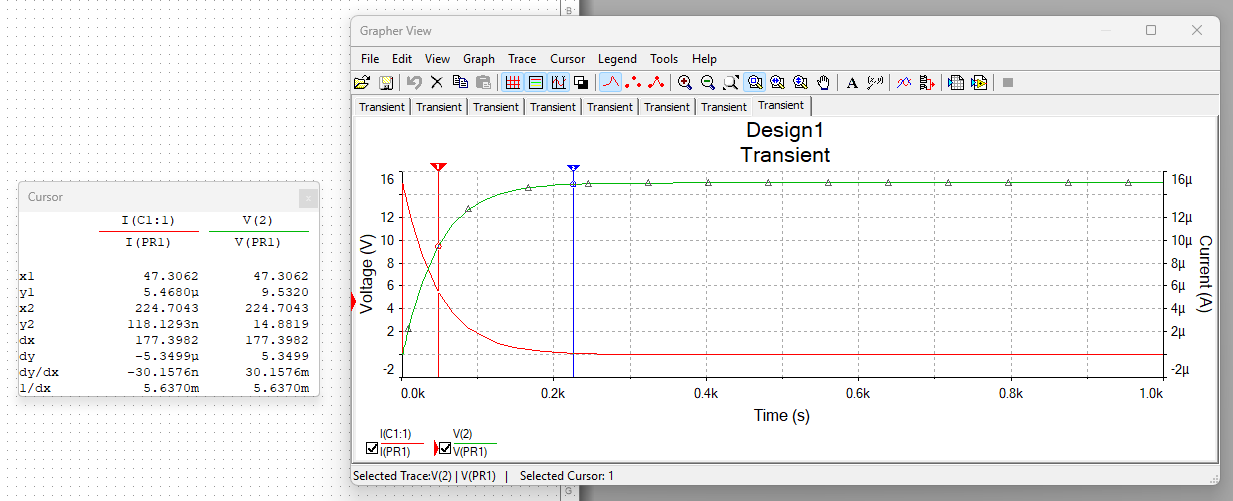
\includegraphics[width=\linewidth]{grapher-circuit1}
  \caption{Multisim's Grapher with Circuit~1's two traces, before the
    export. Cursor~1 at \qty{47.3}{\second} reads \qty{9.532}{\volt} and
    \qty{5.468}{\micro\ampere}.}
  \label{fig:grapher}
\end{marginfigure}%
was moved to a right-hand axis (Figure~\ref{fig:single}). Circuits 2--4 were
then built beside it with each probe renamed to its time constant
(Figure~\ref{fig:ms-charge}), and the analysis was re-run plotting the four
voltages (Figure~\ref{fig:charge-v}) and then the four currents
(Figure~\ref{fig:charge-i}). Instead of reading values off the Grapher's
cursors, each plot was exported to Excel, and the values at \ntau{1} and
\ntau{5} were interpolated between the two nearest exported points.

\widefig{1}{multisim-charge}{Part~II circuits in Multisim. Each AV probe is
  named for its circuit's time constant and points into the capacitor.}{fig:ms-charge}

\begin{figure}
  % Figure 3: Circuit 1 charging, vC on the left axis and iC on the right,
% as in handout step 10. Lines are the formulas, marks the Multisim export
% (data/single-*.dat; t = 0 current set to 15 µA, the export writes 0).
% At 1τ = 47 s: 15(1 - e^-1) = 9.48 V and 15 e^-1 = 5.52 µA; the export,
% interpolated, reads 9.502 V and 5.498 µA.
% Both axes use set layers so the right axis's line (drawn with the second
% axis) goes under the vC trace from the first, as the left one does.
\hspace*{\chartgutter}\begin{tikzpicture}[trim axis left]
  \begin{axis}[labplot, set layers=standard, width=268pt, height=126pt,
      xmin=0, xmax=1000, ymin=0, ymax=16,
      xtick={0,200,...,1000}, ytick={0,4,...,16},
      xlabel={Time (s)}, yticklabel style={text width=14pt, align=right},
      ylabel={V}, ylabel style={rotate=-90, at={(ticklabel cs:1)}, anchor=south, yshift=2pt},
      axis y line*=left]
    % Drawn first so the voltage trace and its 1τ dot sit on top of it
    \draw[level] (axis cs:47,0) -- (axis cs:47,16);
    \addplot[theory=traceInk, domain=0:1000] {15*(1-exp(-x/47))};
    \addplot[export=traceInk, mark=*] table[x=t, y=y] {data/single-v.dat};
    \node[tag, text=chartText, anchor=south west] at (axis cs:47,14.6) {1$\tau$ = \qty{47}{\second}};
    \fill[traceInk] (axis cs:47,9.48) circle[radius=1.8pt];
    \node[note, anchor=west, text=traceInk] at (axis cs:60,9.6) {\qty{9.48}{\volt}};
    \node[tag, text=traceInk, anchor=north east] at (axis cs:990,14.4) {\(v_C\), left axis};
  \end{axis}
  \begin{axis}[labplot, set layers=standard, width=268pt, height=126pt,
      xmin=0, xmax=1000, ymin=0, ymax=16,
      ytick={0,4,...,16}, grid=none,
      axis x line=none, axis y line*=right,
      ylabel={\unit{\micro\ampere}}, ylabel style={rotate=-90, at={(ticklabel cs:1)}, anchor=south, yshift=2pt}]
    \addplot[theory=accent, domain=0:1000] {15*exp(-x/47)};
    \addplot[export=accent, mark=square*] table[x=t, y=y] {data/single-i.dat};
    \fill[accent] (axis cs:47,5.52) circle[radius=1.8pt];
    \node[note, anchor=west, text=accent] at (axis cs:60,5.3) {\qty{5.52}{\micro\ampere}};
    \node[tag, text=accent, anchor=north east] at (axis cs:990,1.8) {\(i_C\), right axis};
  \end{axis}
\end{tikzpicture}

  \caption{Circuit~1 charging: capacitor voltage and current, with
    \ntau{1} = \qty{47}{\second} marked. Lines are calculated values; marks are the
    exported points.}
  \label{fig:single}
\end{figure}

\subsection{Results}

For Circuit~1 alone, the exported data at \qty{47}{\second} reads
\qty{9.502}{\volt} and \qty{5.498}{\micro\ampere}, within
\qty{0.4}{\percent} of the calculated \qty{9.48}{\volt} and
\qty{5.52}{\micro\ampere}. Circuits 2 and~3 agree as closely; Circuit~4 is
the outlier (Table~\ref{tab:charge}).

\begin{table}
  \begin{labtable}{X[0.9]X[0.9]X[1.15]X[1]X[1.15]X[1]X[1.15]}
    Circuit & $\tau$ (\unit{\second}) & \Vc{} at \ntau{1} (\unit{\volt}) & Error (\unit{\percent})
      & \Ic{} at \ntau{1} (\unit{\micro\ampere}) & Error (\unit{\percent}) & \Vc{} at \ntau{5} (\unit{\volt}) \\
    1 & \num{47}    & \num{9.502} & \num{+0.23} & \num{5.498} & \num{-0.39} & \num{14.904} \\
    2 & \num{100}   & \num{9.474} & \num{-0.07} & \num{5.526} & \num{+0.12} & \num{14.900} \\
    3 & \num{147}   & \num{9.486} & \num{+0.06} & \num{5.514} & \num{-0.11} & \num{14.899} \\
    4 & \num{31.97} & \num{9.323} & \num{-1.66} & \num{5.677} & \num{+2.85} & \num{14.909} \\
  \end{labtable}
  \caption{Multisim values at \ntau{1} and \ntau{5} while charging, from the
    exported data. Errors are against the calculated \qty{9.48}{\volt} and
    \qty{5.52}{\micro\ampere}; all four should read \qty{14.90}{\volt} at
    \ntau{5}.}
  \label{tab:charge}
\end{table}

\begin{figure}
  \fourplot{charge-v}{15*(1-exp(-x/\tau))}{0}{16}{0,4,...,16}{0,4,8,12,16}{9.48}
    {at={(0.985,0.05)}, anchor=south east}{V}
  \caption{Capacitor voltage while charging, all four circuits. Each crosses
    \qty{9.48}{\volt} at its own time constant.}
  \label{fig:charge-v}
\end{figure}

\begin{figure}
  \fourplot{charge-i}{15*exp(-x/\tau)}{0}{16}{0,4,...,16}{0,4,8,12,16}{5.52}
    {at={(0.985,0.95)}, anchor=north east}{\unit{\micro\ampere}}
  \caption{Capacitor current while charging. Every circuit starts at
    \qty{15}{\micro\ampere} and falls to \qty{5.52}{\micro\ampere} at its own
    time constant.}
  \label{fig:charge-i}
\end{figure}

Circuit~4 charged fastest and Circuit~3 slowest, the same order as their time
constants: 32, 47, 100, then \qty{147}{\second}
(Figure~\ref{fig:charge-v}). More capacitance takes longer to fill through the
same \qty{1}{\mega\ohm}. All four reached the same voltage after \ntau{5},
\qty{14.90}{\volt} within \qty{0.01}{\volt}; they just took between
\qty{160}{\second} and \qty{735}{\second} to get there.

The currents rank the same way (Figure~\ref{fig:charge-i}). They have to,
because the current is set by the voltage still left across the resistor,
$(\Vs - v_C) / R$. Once the capacitor is \qty{63.2}{\percent} charged, the
current is down to \qty{36.8}{\percent} of its start, and every circuit starts
at \qty{15}{\micro\ampere} because $R$ is the same. In each row of
Table~\ref{tab:charge} the two readings add back to the source:
$\qty{9.502}{\volt} + (\qty{5.498}{\micro\ampere})(\qty{1}{\mega\ohm}) =
\qty{15.000}{\volt}$.

Circuit~4's
\begin{marginfigure}[2pt]
  % Margin figure: why Circuit 4 reads low at 1τ.
% Export points either side of τ = 31.97 s (data/charge-v-32.dat):
%   25.6 s -> 8.306 V,  45.6 s -> 11.496 V
% Straight line at 31.97 s: 8.306 + (11.496 - 8.306)(6.37/20) = 9.322 V
% Formula: 15(1 - e^-1) = 9.482 V; gap 0.160 V (-1.7 % of 9.48 V)
\begin{tikzpicture}
  \begin{axis}[labplot, width=128pt, height=104pt,
      xmin=20, xmax=50, ymin=7.5, ymax=12,
      xtick={20,30,40,50}, xticklabels={20,30,40,50\,\unit{\second}},
      ytick={8,9,10,11,12}, yticklabels={8,9,10,11,12\,\unit{\volt}}]
    \addplot[theory=tauA, domain=20:50] {15*(1-exp(-x/31.97))};
    \addplot[accent, line width=0.6pt, densely dashed] coordinates {(25.6,8.306) (45.6,11.496)};
    \addplot[export=tauA, mark=*, mark size=1.8pt] coordinates {(25.6,8.306) (45.6,11.496)};
    \draw[chartText, densely dotted, line width=0.4pt] (axis cs:31.97,7.5) -- (axis cs:31.97,12);
    \draw[tauA, line width=0.7pt, fill=white] (axis cs:31.97,9.482) circle[radius=2pt];
    \fill[accent] (axis cs:31.97,9.322) circle[radius=1.6pt];
    \node[note, anchor=south east, text=tauA] at (axis cs:31.2,9.55) {formula\\\qty{9.48}{\volt}};
    \node[note, anchor=north west, text=accent] at (axis cs:32.8,9.25) {straight line\\\qty{9.32}{\volt}};
    \node[note, anchor=north, fill=white] at (axis cs:31.97,7.95) {1$\tau$};
    \node[note, anchor=east, text=tauA] at (axis cs:44.6,11.62) {export};
    \node[note, anchor=south east, text=tauA] at (axis cs:25.4,8.4) {export};
  \end{axis}
\end{tikzpicture}

  \caption{Circuit~4 near its \ntau{1}. The export's nearest points are
    \qty{20}{\second} apart, and the straight line between them passes
    \qty{0.16}{\volt} under the curve at \qty{31.97}{\second}.}
  \label{fig:interp}
\end{marginfigure}%
error is in the export's point spacing, not the circuit. With TSTOP =
\qty{1000}{\second}, Multisim saved points \qty{20}{\second} apart after the
first \qty{25}{\second} (\qty{25.6}{\second}, \qty{45.6}{\second},
\qty{65.6}{\second} and so on), so the export has no point at Circuit~4's
\ntau{1} of \qty{32}{\second}. Its value there comes from a straight line
between the points at \qty{25.6}{\second} and \qty{45.6}{\second}, and a
\qty{20}{\second} gap is almost two-thirds of its $\tau$, so the line cuts
under the curve (Figure~\ref{fig:interp}). The saved points themselves are
within \qty{0.1}{\volt} of the formula. For Circuits 1--3 the same gap is a
smaller fraction of $\tau$, and the error stays under \qty{0.4}{\percent}.

% =====================================================================
\section{Part III: RC Transient Response (Discharge)}

With the sources removed and every capacitor starting at \qty{15}{\volt}, each
voltage falls to \qty{36.8}{\percent} at its own time constant. The readings
mirror Part~II: every \ntau{1} voltage is \qty{15}{\volt} minus its charging
value, and Circuit~3 again takes the longest and Circuit~4 the shortest.

\subsection{Multisim}

The Part~II file was saved as a copy, the four sources were removed, and each
\qty{1}{\mega\ohm} was moved across its capacitor as the discharge path
(Figure~\ref{fig:ms-discharge}). An initial condition on each capacitor takes
the place of the charging step: \qty{15}{\volt} on Circuits 1--3, including
both capacitors in Circuit~3, since parallel capacitors share the same
voltage.

Circuit~4's two capacitors are in series, so they hold the same charge, and
the \qty{15}{\volt} splits between them in inverse proportion to capacitance:
\begin{gather}
  Q = \Ceq\Vs = (\qty{31.97}{\micro\farad})(\qty{15}{\volt}) = \qty{0.480}{\milli\coulomb} \\
  V_{\qty{100}{\micro\farad}} = \frac{\qty{0.480}{\milli\coulomb}}{\qty{100}{\micro\farad}} = \qty{4.80}{\volt}
  \qquad
  V_{\qty{47}{\micro\farad}} = \frac{\qty{0.480}{\milli\coulomb}}{\qty{47}{\micro\farad}} = \qty{10.20}{\volt}
\end{gather}

The smaller capacitor takes the larger share, and the two add back to
\qty{15}{\volt}. The analysis was re-run to \qty{1000}{\second}, plotting the
four voltages (Figure~\ref{fig:discharge-v}) and then the four currents
(Figure~\ref{fig:discharge-i}). The probes were left as in Part~II, so the
current now flows out of the capacitor against the arrow and reads negative.

\widefig{1}{multisim-discharge}{Part~III circuits in Multisim. The sources are
  gone, each \qty{1}{\mega\ohm} sits across its capacitor, and the initial
  conditions (IC) stand in for the charge. Circuit~4's \qty{4.8}{\volt} and
  \qty{10.2}{\volt} add to \qty{15}{\volt}.}{fig:ms-discharge}

\subsection{Results}

\begin{table}
  \begin{labtable}{X[0.9]X[0.9]X[1.15]X[1]X[1.15]X[1]X[1.15]}
    Circuit & $\tau$ (\unit{\second}) & \Vc{} at \ntau{1} (\unit{\volt}) & Error (\unit{\percent})
      & \Ic{} at \ntau{1} (\unit{\micro\ampere}) & Error (\unit{\percent}) & \Vc{} at \ntau{5} (\unit{\volt}) \\
    1 & \num{47}    & \num{5.498} & \num{-0.39} & \num{-5.498} & \num{-0.39} & \num{0.095} \\
    2 & \num{100}   & \num{5.526} & \num{+0.12} & \num{-5.526} & \num{+0.12} & \num{0.100} \\
    3 & \num{147}   & \num{5.514} & \num{-0.11} & \num{-5.514} & \num{-0.11} & \num{0.101} \\
    4 & \num{31.97} & \num{5.677} & \num{+2.85} & \num{-5.677} & \num{+2.85} & \num{0.091} \\
  \end{labtable}
  \caption{Multisim values at \ntau{1} and \ntau{5} while discharging, from
    the exported data. Errors are against the calculated \qty{5.52}{\volt} and
    \qty{5.52}{\micro\ampere}, current by magnitude; all four should read about
    \qty{0.10}{\volt} at \ntau{5}.}
  \label{tab:discharge}
\end{table}

\begin{figure}
  \fourplot{discharge-v}{15*exp(-x/\tau)}{0}{16}{0,4,...,16}{0,4,8,12,16}{5.52}
    {at={(0.985,0.95)}, anchor=north east}{V}
  \caption{Capacitor voltage while discharging. Each falls to
    \qty{5.52}{\volt} at its own time constant.}
  \label{fig:discharge-v}
\end{figure}

\begin{figure}
  \fourplot{discharge-i}{-15*exp(-x/\tau)}{-16}{0}{-16,-12,...,0}{−16,−12,−8,−4,0}{-5.52}
    {at={(0.985,0.05)}, anchor=south east}{\unit{\micro\ampere}}
  \caption{Capacitor current while discharging. Each starts at
    \qty{-15}{\micro\ampere}, negative because the current now leaves the
    capacitor against the probe arrow.}
  \label{fig:discharge-i}
\end{figure}

Circuit~3 took the longest to discharge and Circuit~4 the shortest
(Figure~\ref{fig:discharge-v}), the same order as charging and for the same
reason. More capacitance holds more charge at \qty{15}{\volt}, and the same
\qty{1}{\mega\ohm} drains it no faster than \qty{15}{\micro\ampere}.

The current curves rank the same way (Figure~\ref{fig:discharge-i}), and they
have to: with only the \qty{1}{\mega\ohm} in the loop, the current is the
capacitor voltage divided by \qty{1}{\mega\ohm}.\sidenote{One volt across
\qty{1}{\mega\ohm} drives one microamp, so for these circuits volts and
microamps are the same number.} Each current curve is its voltage curve
flipped negative, which is why the readings in \unit{\micro\ampere} match the
readings in volts in every row of Table~\ref{tab:discharge}.

Each \ntau{1} reading is the Part~II value turned over,
$\qty{5.498}{\volt} = \qty{15}{\volt} - \qty{9.502}{\volt}$ for Circuit~1 and
likewise for the rest. Charging and discharging follow the same exponential,
one rising toward \qty{15}{\volt} and the other falling toward \qty{0}{\volt}.
Circuit~4's \qty{+2.85}{\percent} is the same \qty{20}{\second} point spacing
as in Part~II. At \ntau{5} it reads \qty{0.091}{\volt} against about
\qty{0.10}{\volt}, but a percent error on a value that small mostly measures
the interpolation.

\end{document}
